\documentclass[../Report.tex]{subfiles}

\begin{document}


\chapter{Test}
\label{chap:test}
---- In diesem Kapitel werden die Rahmen / Start-Bedingungen des Seminars vorgestellt.  --- 

\section{---- firstName ----}
\label{sec:test_firstName}
--- in dieser section wird das BB-Signal nochmals kurz erläutert und eine allgemeine Erläuterung gegeben ---
--- Ziel des Abschnitts: Leser hat grobe Vorstellung, in welchem Kontext unser Programm entstanden ist und eingesetzt wird \\ Diese Zeile teste das paket $ nameref$ mit \nameref{chap:test} und hier mit einer PHANTOMSECTION via \nameref{pha:test.try}---

%\begin{figure}[htb]
%\begin{center}
%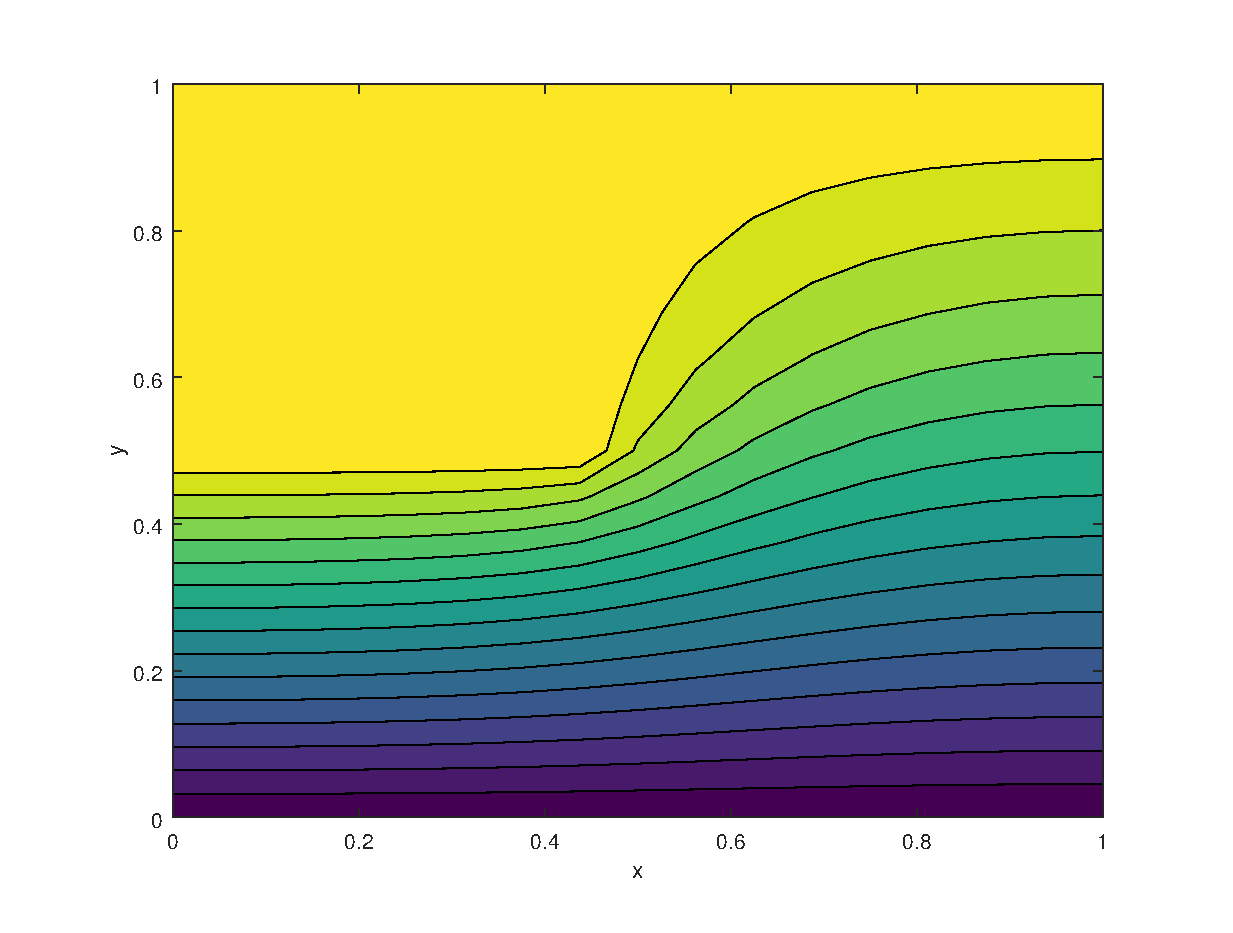
\includegraphics[scale=0.6]{eps/plotPot}
%\end{center}
%\caption[Potentialverlauf eines Kondensators mit Kante]{Potentialverlauf des Kondensators mit Kante.}
%\label{fig:V4.PA4.1}
%\end{figure}

\begin{figure}
	\centering
	\begin{tikzpicture}[scale=1]
		\begin{axis}[
		xlabel={x},
		ylabel={mode},
		%grid=major,
		cycle multi list={color list\nextlist [1 of]mark list},
		legend entries={Grundmode},
		legend style={at={(0.5,-0.2)},anchor=south},
		]
		\addplot table[x=x, y=mode1, col sep=comma] {../csv/modes.csv};
		\addplot+
%		\addplot+ [
%mark=ball,
%mark size=4pt,
%scatter,% enable scatter
%scatter src=rand,% the "color data"
%% configure individual appearances:
%scatter/use mapped color=
%{ball color=mapped color}]
coordinates
{(-0.1,0) (-1,0.1) (0,0) (0.1,0.1) (0.2,0)};

		
		
		\end{axis}
	\end{tikzpicture}
	\caption{asdf}
\end{figure}



\pgfplotstableread[col sep = comma, columns/3/.style={string type}, ignore chars= {(, ),j}] {transfer_fct.csv}\kennlinie %%%%% cannot deal with a 'j' in imaginary part! %%%
%\pgfplotstabletypeset[columns={0,3}, columns/3/.style={string type}] \kennlinie
% erzeugt eine banale Liste

\begin{figure}[hb]
\centering
    \begin{tikzpicture}
\begin{axis}[
		legend entries = {Amplitude},
		legend pos = outer north east,
		]
\addplot[blue, thick] table [ x =0, y index=1] {\kennlinie};

		\addplot [red, mark=o, mark size=5pt]coordinates {(10000000, 8)};
		\addplot coordinates{(20000000, 5)}	;	
		
\end{axis}
\end{tikzpicture}
\caption{Einzelsinus}
\end{figure}

Dies ist ein Versuch, eine Transfer-Function zu plotten mittels tikz:

%\begin{figure}[h!]
%\centering
%    \begin{tikzpicture}
%    \datavisualization [scientific axes=clean, 
%    					visualize as line, 
%    					x axis = {attribute = frequency},
%    					y axis = {attribute = amplitude}]
%    	data [read from file = transfer_fct.csv,
%    			%headline = {frequency, amplitude, phaseshift, complex}
%    			];
%    
    
%\begin{axis}[grid=both, xlabel={$t/T_{\textrm{BB}}$},
%ylabel={$\Usin(t)$},                        ytick={-1,1},
%                        yticklabels={$-\widehat{U}$,$\widehat{U}$},
%                        xtick={-4,-2,0,2,4},
%                        xticklabels={-2,-1,0,1,2}]
%\addplot[blue, thick] table [ x expr={\thisrowno{0}}, y
%expr={\thisrowno{1}}, col sep=semicolon] {csv/transfer_fct.csv};
%\end{axis}
%	\end{tikzpicture}
%\caption{Bsp-Plot einer Transfer-Function H}
%  \label{fig:bsp_transfer}
%\end{figure}


Dies ist ein Versuch, ein Frequenzspektrum zu plotten und Marker an relevanten Punkten zu setzen:




\end{document}